%yright 2007, 2008, 2009 Elsevier Ltd
%% 
%% This file is part of the 'Elsarticle Bundle'.
%% ---------------------------------------------
%% 
%% It may be distributed under the conditions of the LaTeX Project Public
%% License, either version 1.2 of this license or (at your option) any
%% later version.  The latest version of this license is in
%%    http://www.latex-project.org/lppl.txt
%% and version 1.2 or later is part of all distributions of LaTeX
%% version 1999/12/01 or later.
%% 
%% The list of all files belonging to the 'Elsarticle Bundle' is
%% given in the file `manifest.txt'.
%% 

%% Template article for Elsevier's document class `elsarticle'
%% with numbered style bibliographic references
%% SP 2008/03/01

% \documentclass[preprint,11pt]{elsarticle}
\documentclass[final,1p,11pt]{elsarticle}

%\documentclass[final,1p,times]{elsarticle}


%% Use the option review to obtain double line spacing
%%\documentclass[authoryear,preprint,review,12pt]{elsarticle}

%% Use the options 1p,twocolumn; 3p; 3p,twocolumn; 5p; or 5p,twocolumn
%% for a journal layout:
%% \documentclass[final,1p,times]{elsarticle}
%% \documentclass[final,1p,times,twocolumn]{elsarticle}
%% \documentclass[final,3p,times]{elsarticle}
%% \documentclass[final,3p,times,twocolumn]{elsarticle}
%% \documentclass[final,5p,times]{elsarticle}
%% \documentclass[final,5p,times,twocolumn]{elsarticle}

%%% For including figures, graphicx.sty has been loaded in
%% elsarticle.cls. If you prefer to use the old commands
%% please give \usepackage{epsfig}


\usepackage{epsfig}
%\usepackage{cite}
%\usepackage{mcite}
\usepackage{array,tabularx,epsfig,mathrsfs,graphicx,rotating}
\usepackage{ifthen}
\usepackage{amsfonts}
\usepackage{ragged2e}
\PassOptionsToPackage{hyphens}{url}
\usepackage[hyphens]{url}
\usepackage{hyperref}
\usepackage{listings}
\usepackage{lineno}
\usepackage{subfigure}
\usepackage{epstopdf}
% Custom colors
\usepackage{color}
\usepackage{float}
\usepackage{verbatim}
\usepackage{color,soul}

% to cross text
\usepackage[normalem]{ulem} % either use this (simple) or
\usepackage{soul} % use this (many fancier options)
\usepackage{amsmath,amssymb}

\let\originallesssim\lesssim
\let\originalgtrsim\gtrsim

\DeclareRobustCommand{\lesssim}{%
  \mathrel{\mathpalette\lowersim\originallesssim}%
}
\DeclareRobustCommand{\gtrsim}{%
  \mathrel{\mathpalette\lowersim\originalgtrsim}%
}

\makeatletter
\newcommand{\lowersim}[2]{%
  \sbox\z@{$#1<$}%
  \raisebox{-\dimexpr\height-\ht\z@}{$\m@th#1#2$}%
}
\makeatother


\hypersetup{
  colorlinks=true,
  linkcolor=blue,
  citecolor=blue,
  urlcolor=blue
}




\graphicspath{{figs/}}


\pdfinfo{
   /Author (Chekanov et al)
   /Title  (Studies of granularity of a hadronic calorimeter for tens-of-TeV jets  at a 100 TeV pp collider)
   /CreationDate (D:2017)
   /Subject (PDFLaTeX)
   /Keywords (PDF;LaTeX)
}


\textheight=22cm
\textwidth=14.5cm

\newcommand{\beq}{\begin{equation}}
\newcommand{\eeq}{\end{equation}}
\newcommand{\la}{\langle}
\newcommand{\promc}{{\sc ProMC}}
\newcommand{\ra}{\rangle}
\newcommand{\eps}{\epsilon}
\newcommand{\ud}{\mathrm{d}}
\newcommand{\Ec}{\mathcal{E}}
\newcommand{\Fc}{\mathcal{F}}
\newcommand{\Za}{\mathrm{Z_1}}
\newcommand{\Zb}{\mathrm{Z_2}}
\newcommand{\Zn}{\mathrm{Z_n}}
\newcommand{\F}{\mathrm{F}}

\chardef\til=126
\newcommand{\GEANTfour} {\textsc{geant4}}
\newcommand{\pythia} {\textsc{Pythia8~}}
\newcommand{\pt}{\ensuremath{p_{\mathrm{T}}}}


\journal{}

\begin{document}
%\hfill ANL-HEP-149528
\definecolor{mygreen}{rgb}{0,0.6,0} \definecolor{mygray}{rgb}{0.5,0.5,0.5} \definecolor{mymauve}{rgb}{0.58,0,0.82}

\lstset{ %
 backgroundcolor=\color{white},   % choose the background color; you must add \usepackage{color} or \usepackage{xcolor}
 basicstyle=\footnotesize,        % the size of the fonts that are used for the code
 breakatwhitespace=false,         % sets if automatic breaks should only happen at whitespace
 breaklines=true,                 % sets automatic line breaking
 captionpos=b,                    % sets the caption-position to bottom
 commentstyle=\color{mygreen},    % comment style
 deletekeywords={...},            % if you want to delete keywords from the given language
 escapeinside={\%*}{*)},          % if you want to add LaTeX within your code
 extendedchars=true,              % lets you use non-ASCII characters; for 8-bits encodings only, does not work with UTF-8
 keepspaces=true,                 % keeps spaces in text, useful for keeping indentation of code (possibly needs columns=flexible)
 frame=tb,
 keywordstyle=\color{blue},       % keyword style
 language=Python,                 % the language of the code
 otherkeywords={*,...},            % if you want to add more keywords to the set
 rulecolor=\color{black},         % if not set, the frame-color may be changed on line-breaks within not-black text (e.g. comments (green here))
 showspaces=false,                % show spaces everywhere adding particular underscores; it overrides 'showstringspaces'
 showstringspaces=false,          % underline spaces within strings only
 showtabs=false,                  % show tabs within strings adding particular underscores
 stepnumber=2,                    % the step between two line-numbers. If it's 1, each line will be numbered
 stringstyle=\color{mymauve},     % string literal style
 tabsize=2,                        % sets default tabsize to 2 spaces
 title=\lstname,                   % show the filename of files included with \lstinputlisting; also try caption instead of title
 numberstyle=\footnotesize,
 basicstyle=\small,
 basewidth={0.5em,0.5em}
}


\begin{frontmatter}

\title{
Physics potential of timing layers for future detectors}
%%%%%%%%%%%%%%%%%%%%%%%%%%%%%%%%%%%%%%%%%%%%%%%%%%%%%%%%%%%%%%%

\author[add3]{C.-H. Yeh}
\ead{a9510130375@gmail.com}

\author[add1]{S.V.~Chekanov}
\ead{chekanov@anl.gov}

\author[addDuke]{A.V.~Kotwal}
\ead{ashutosh.kotwal@duke.edu}

\author[add2]{N.V.~Tran}
\ead{ntran@fnal.gov}

\author[add3]{S.-S.~Yu}
\ead{syu@cern.ch}

\address[add3]{
Department of Physics and Center for High Energy and High Field Physics, 
National Central University, Chung-Li, Taoyuan City 32001, Taiwan
}

\address[add1]{
HEP Division, Argonne National Laboratory,
9700 S.~Cass Avenue,
Argonne, IL 60439, USA. 
}

\address[addDuke]{
Department of Physics, Duke University, USA
}

\address[add2]{
Fermi National Accelerator Laboratory
}




\begin{abstract}

\end{abstract}

\begin{keyword}

\end{keyword}
\end{frontmatter}



%%%%%%%%%%%%%%%%%%%%%%%%%%%%%%%%%%%%%%%%%%%%%%%%%%%%%%%%%%%%%%%%%%
\section{Introduction}

Future experiments, such as CLIC \cite{Linssen:1425915}, International Linear Collider (ILC) \cite{Behnke:2013xla}, high-energy LHC (HE-LHC),
future circular $pp$ colliders of the European initiative, FCC-hh~\cite{Benedikt:2206376} and the Chinese initiative, SppC~\cite{Tang:2015qga} will require high precision measurements of particle and jets 
at large transverse momenta. 
The usage of timing information for such experiments  can  provide additional 
information that can be used to improve particle and jet reconstruction, as well as to deal with background events.
At this moment, conceptional design reports for these experiments did not fully explore
the benefits of the time of flight (TOF) measurements with tens-of-picosecond resolutions.

\section{Proposal}

A generic design of hadronic (electromagnetic) calorimeters for future particle collision experiments (HE-LHC, FCC, CLIC, ILC etc.) 
is based on two main characteristics: (1) high-granularity calorimeters with cells ranged from $3\times 3$ mm$^2$ (for ECAL) to $5\times 5$ cm$^2$  (for HCAL) in sizes.
(2) timing with nanosecond precision that improves background rejection, vertex association, and detection of new particles. 
According to the CPAD report \cite{Ahmed:2019sim}, a development of “picosecond time resolution” for future calorimeters is one of the critical needs. 
Presently. high-granularity calorimeters (with >1 millions channels) with tens of picoseconds resolution represent a 
significant challenge due the large cost.

As a part of the HL-LHC upgrade program, CMS and ATLAS experiments are designing high-precision timing detectors with the time resolution of about 30 ps. 
They are based on silicon sensors that add an extra ``dimension’’ to event reconstruction. 
Such timing capabilities are not fully explored for future detectors beyond the HL-LHC upgrade. 
High-precision timing will be beneficial for new physics searches and b-tagging for all post-LHC experiments. 
For CLIC and FCC, high-precision time stamping will be essential for background rejection and pile-up mitigation. 

Currently, the baseline designs of the high-granularity ECAL and HCAL of the CLIC/FCC detectors have not been 
optimized for precision timing in the range of a few tens of picoseconds. 
The latter is considered as an expensive option for many mullions of channels of these high-granularity detectors. 
This opens an opportunity to investigate a cost-effective “timing layer” (with the time resolution of smaller than 30~ps) for the post-LHC detectors. 
This layer will be installed on front of high-granularity calorimeters, covering both the forward and barrel regions.

In this paper we  will investigate physics advantages for timing layers in the front of calorimeters  
of the post-LHC experiments. 
Typically, thin detectors on front of calorimeters are called ``preshower''. The design goal of such detectors is to count the number of charged
particles in oder to correct for energy loses. The timing information of ``mips'' ( minimum–ionising particles) is not used for particle identifications. 
Unlike the standard pre-shower detector, we propose not only count mips, but also reconstruct high-precision timing and the position.
This timing detector will have a similar granularity as the proposed high-granularity EM calorimeters themselves, 
but will have a sensor technology and readout which is best suited for mip time stamping (not necessarily for energy reconstruction). 
Our proposal is to enclose the EM detectors with two timing layers, one - before the first EM layer, and the second is after the last EM layer (but before
the HCAL). The two layers of the timing detector allows a robust identification of time by correlating the position and timestamps of the particle passing through
the ECAL.

In this paper we will explore this idea using full Monte Carlo simulations. 
A schematic representation of the positions of the timing layers for a generic detector geometry is shown in Fig.~\ref{fig:eff_rad}



\begin{figure}
\begin{center}
   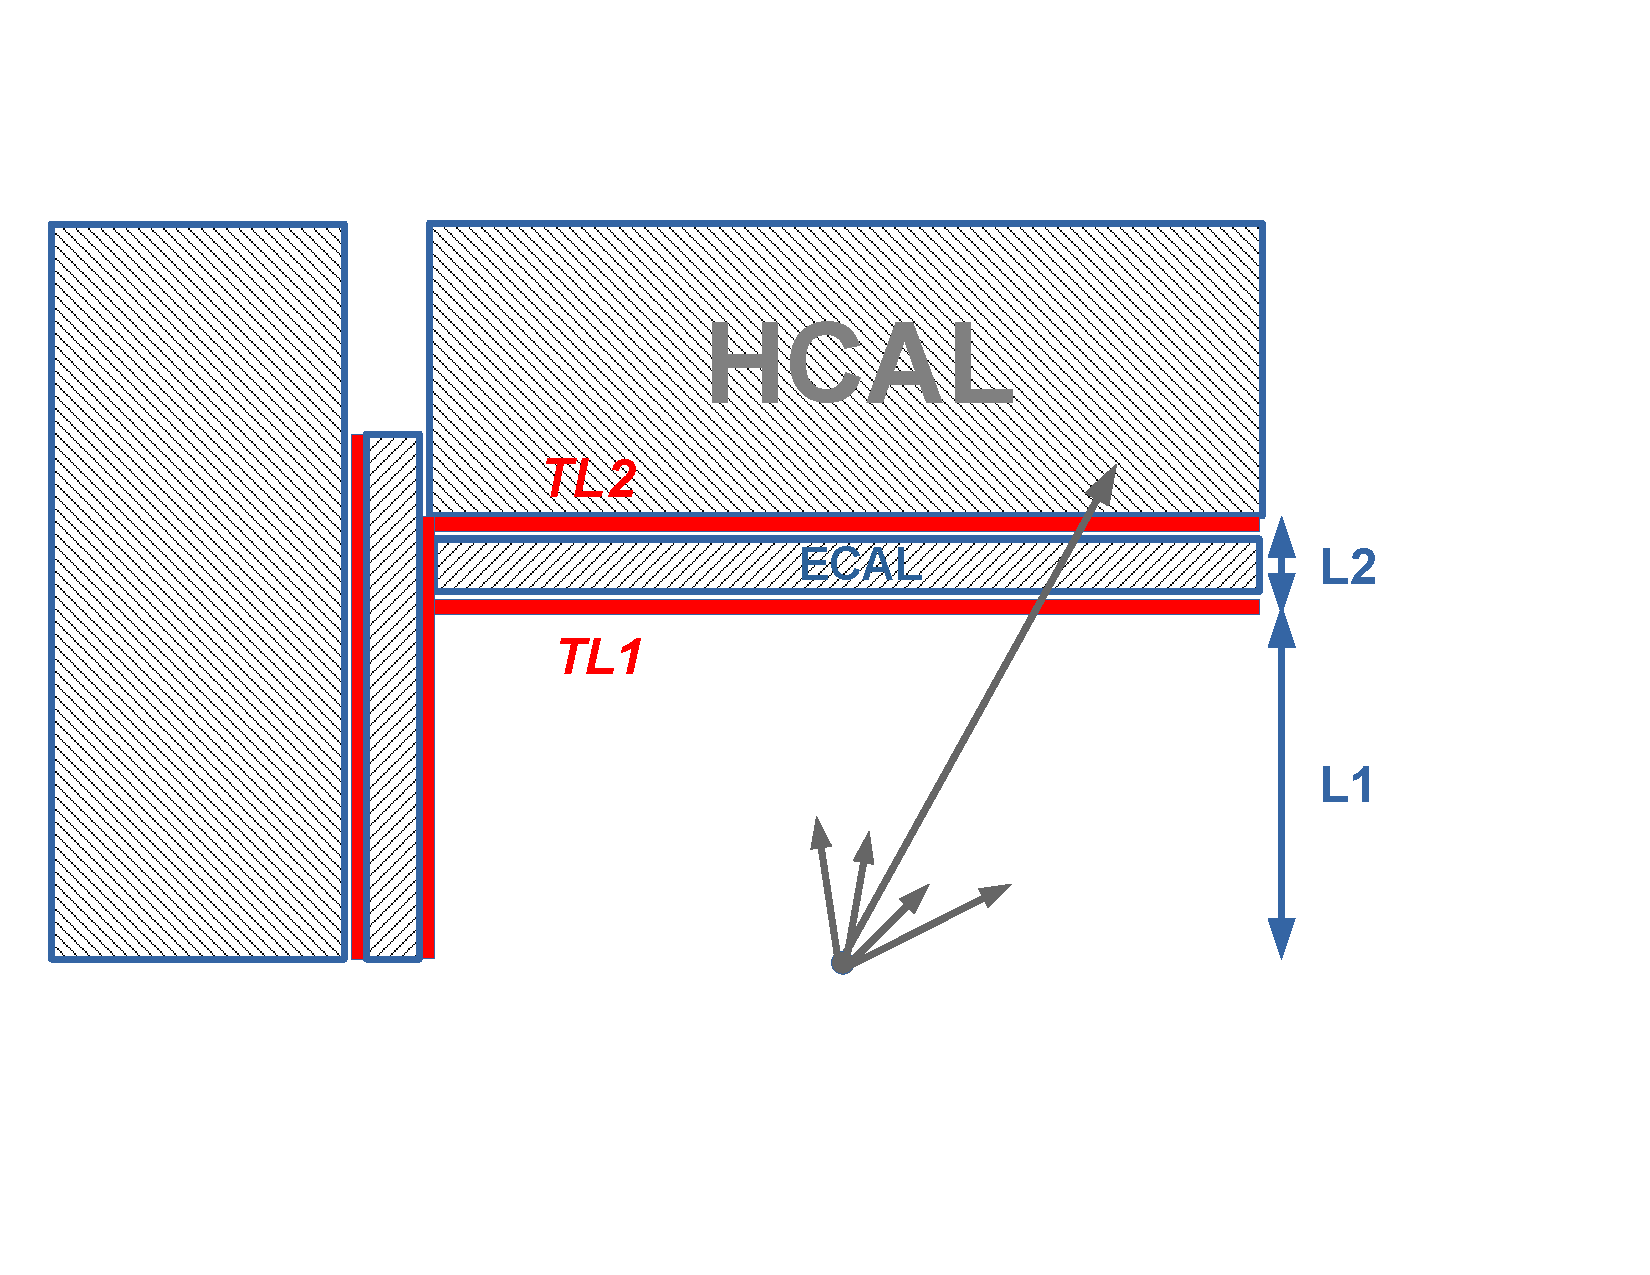
\includegraphics[width=0.8\textwidth]{timing_layer.pdf}\hfill
\end{center}
\caption{An example of positions of the thin timing layers for a generic detector. The thin timing layers  will enclose the electromagnetic calorimeter, allow a reliable reconstruction of the  mip signals with a timing resolution of the order of 10~ps.}
\label{fig:eff_rad}
\end{figure}


The second layer of the timing detector can be justified if fluctuations of hits times are smaller than  the resolution 
of the timing layers. In oder to verify this, we used a full Geant4 (version 10.3)~\cite{Allison2016186} simulation 
of the SiFCC detector \cite{Chekanov:2016ppq} that allows to use the information on hits from the ECAL.
The ECAL is built from a highly segmented silicon-tungsten  with the transverse cell size of $2 \times 2$~cm.
The ECAL has 30 layers built from tungsten pads with silicon readout,
corresponding to 35~X$_{0}$. The first 20 layers use tungsten of 3~mm thickness.
The last ten layers use tungsten layers of
twice the thickness, and thus have half the  sampling fraction.  

To verify that the time differences between last and first layer of ECAL is sufficiently small, and can be neglected for the timing layers that
have a timing resolution of the order of 10~ns, a sample of single pions was created with 1 and 10~GeV momenta. 
The particles were reconstructed in the ECAL calorimeter,
and the time difference $\Delta T= T_{\mathrm{last}}-T_{\mathrm{first}}$ of the hits between the last and first ECAL layers was calculated.
Only hits that arrive first were considered.
Figure~\ref{fig:timediff} shows the time distribution for 1 and 10 GeV pions. It can be seen that the peak positions of the distributions are smaller
than 1~ps, as expected for the distance of about 20~cm between  the last and first layers\footnote{The precision with which the simulations were performed are about 0.2-0.3~ns}. More importantly, the RMS of these distributions are significantly smaller than the 10~ns. 
Therefore, for the timing layers that have a resolution of the order of 10-20~ns, a single particle crossing the two layers  will be seen a single simultaneous hit,
thus such hits can be well correlated in time and identified as a single crossing particle.
 

\begin{figure}
\begin{center}
   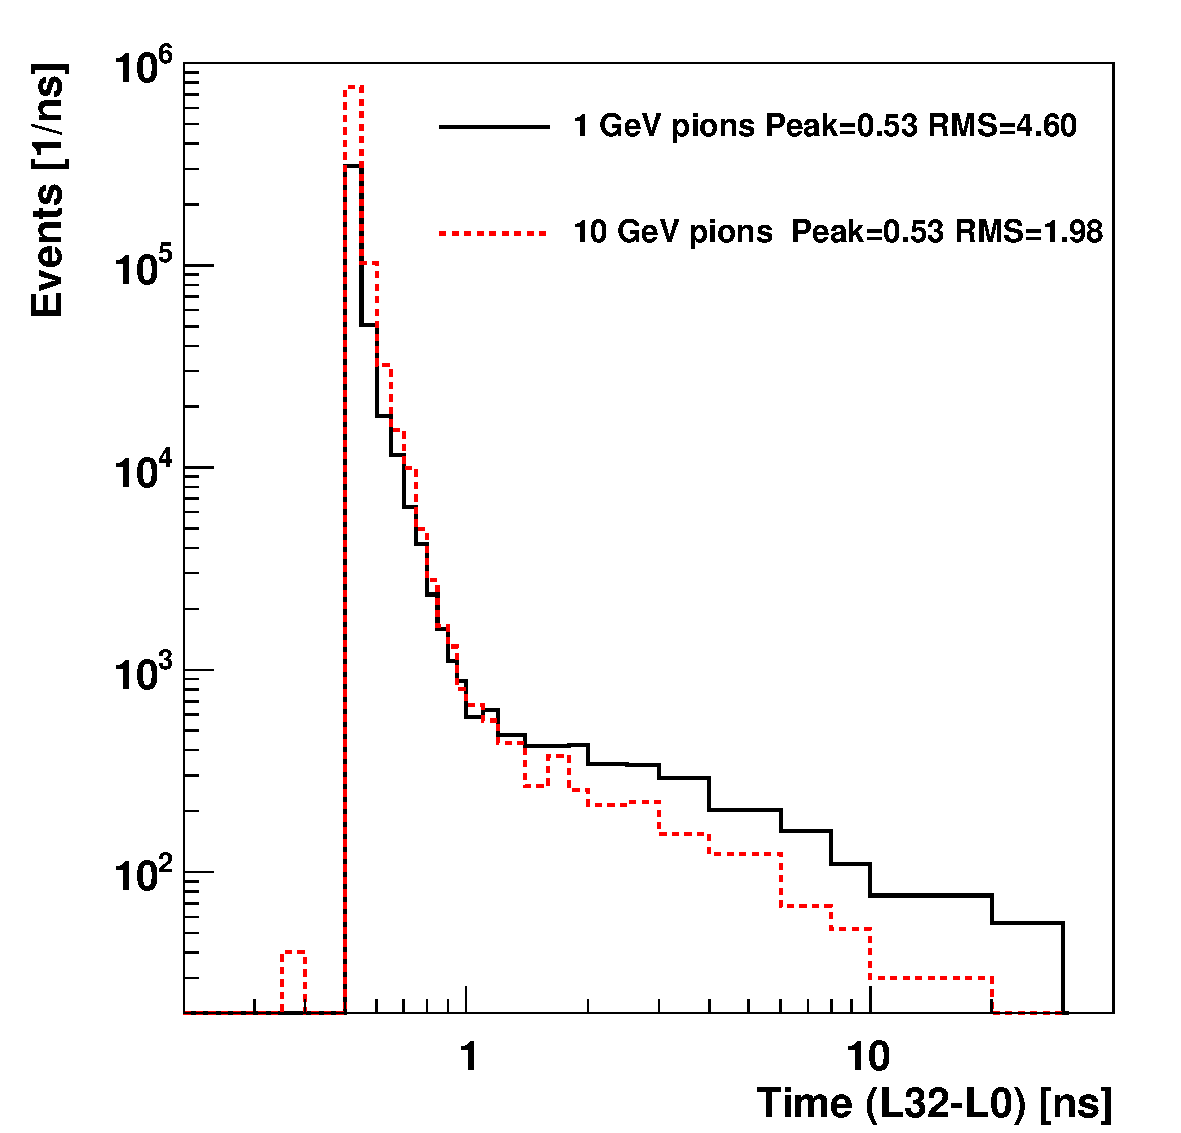
\includegraphics[width=0.6\textwidth]{timeECAL_2layers1.pdf}\hfill
\end{center}
\caption{The difference between time of hits between the last and first layer of ECAL for single pions with the transverse momentum 1 and 10 GeV. 
Only first (fastest) hits were considered}
\label{fig:timediff}
\end{figure}



\clearpage 
%%%%%%%%%%%%%%%%%%%%%%%%%%%%%%%%%%%%%%%%%%%%%%%%%%%%%%%%%%%%%%%%%%

%%%%%%%%%%%%%% sections 
\section{Timing layers for single particles}

Now we discuss the kinematic regions  relevant for  TOF measurements of SM and BSM particles. Instead of the full {\sc geant}4 simulations, we will
use a semi-analytic approach.  
 
To estimate the separation power between different mass hypotheses, we calculate the mass and momentum for which one can achieve a separation 
 significance higher than $3\sigma$ (or p-value$<0.3$\%). 
If there are two particles with mass $m$ and a reference (fixed) mass $m_F$, respectively, the $3\sigma$ separation can be 
achieved for this condition~\cite{Cerri:2018rkm}:
\begin{equation}
\frac{L}{c \sigma_{\textsc{TOF}}}\left|\sqrt{1+\frac{m^2}{p^2}} - \sqrt{1+\frac{m_F^2}{p^2}}\right| > 3
\label{eqTOF}
\end{equation}
where $p$ is the momentum of a particle with mass $m$, $L$  is the length of the particle's trajectory, 
and $\sigma_{TOF}$ is the
resolution  of the timing layer that measures the TOF.

Figure~\ref{fig:singleparticles} shows the $3\sigma$ separation from the pion
mass hypothesis ($m_F=m_{\pi}$) using the procedure discussed  in~\cite{Cerri:2018rkm}. The 
calculations are performed for several values of resolution of the timing layer, ranging from 10~ps to 1~ns,
as a function of $L$ and $p$. For a 20~ps detector and a typical travel 
distance $L\sim 1.5-2$~m from the production vertex to the ECAL, neutrons and protons can be separated from the pion hypothesis up to $p \approx 7$~GeV. 
The separation of kaons from pions can be performed up to 3~GeV.
This momentum range should be sufficient for a reliable particle 
identification in a momentum range adequate for some physics studies focused on
single-particle reconstruction (such as B-meson physics).
This can also be used for jets that are dominated
by particles in this momentum range.
For a detector  with 1~ns resolution, the separation can only be possible  up to  300 -- 500~MeV. This is smaller than the 
minimum particle momentum of $\approx$0.5~GeV considered for high-energy proton colliders.
Therefore, a timing layer with 1~ns resolution cannot be used for particle identification in such experiments.

\begin{figure}
\begin{center}
   \subfigure[Neutrons] {
   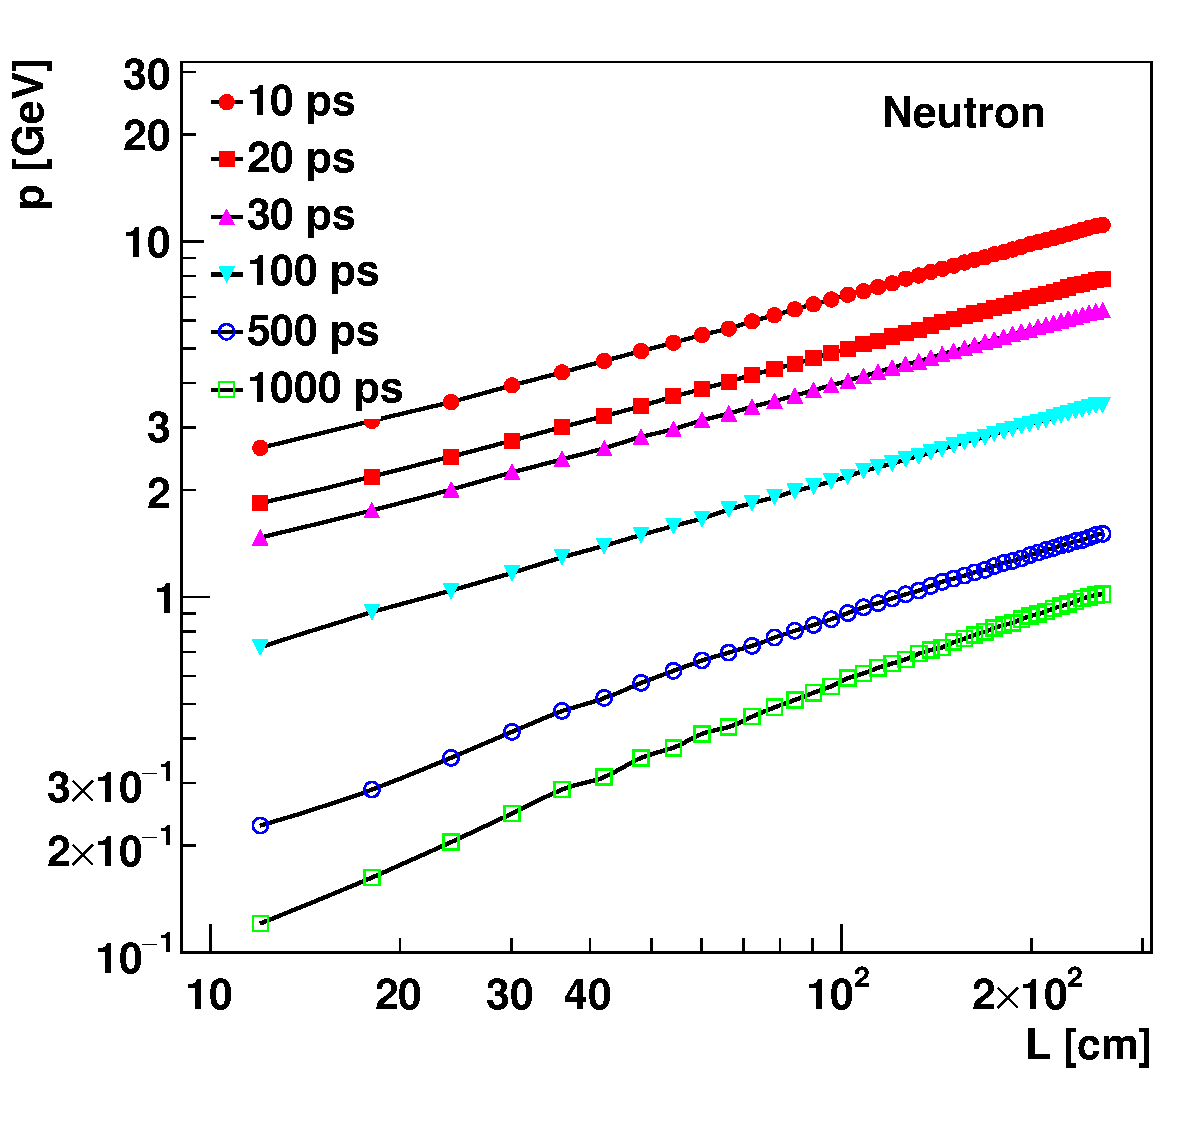
\includegraphics[width=0.45\textwidth]{time_flight_length_neutron.pdf}
   }
      \subfigure[$K$-mesons] {
   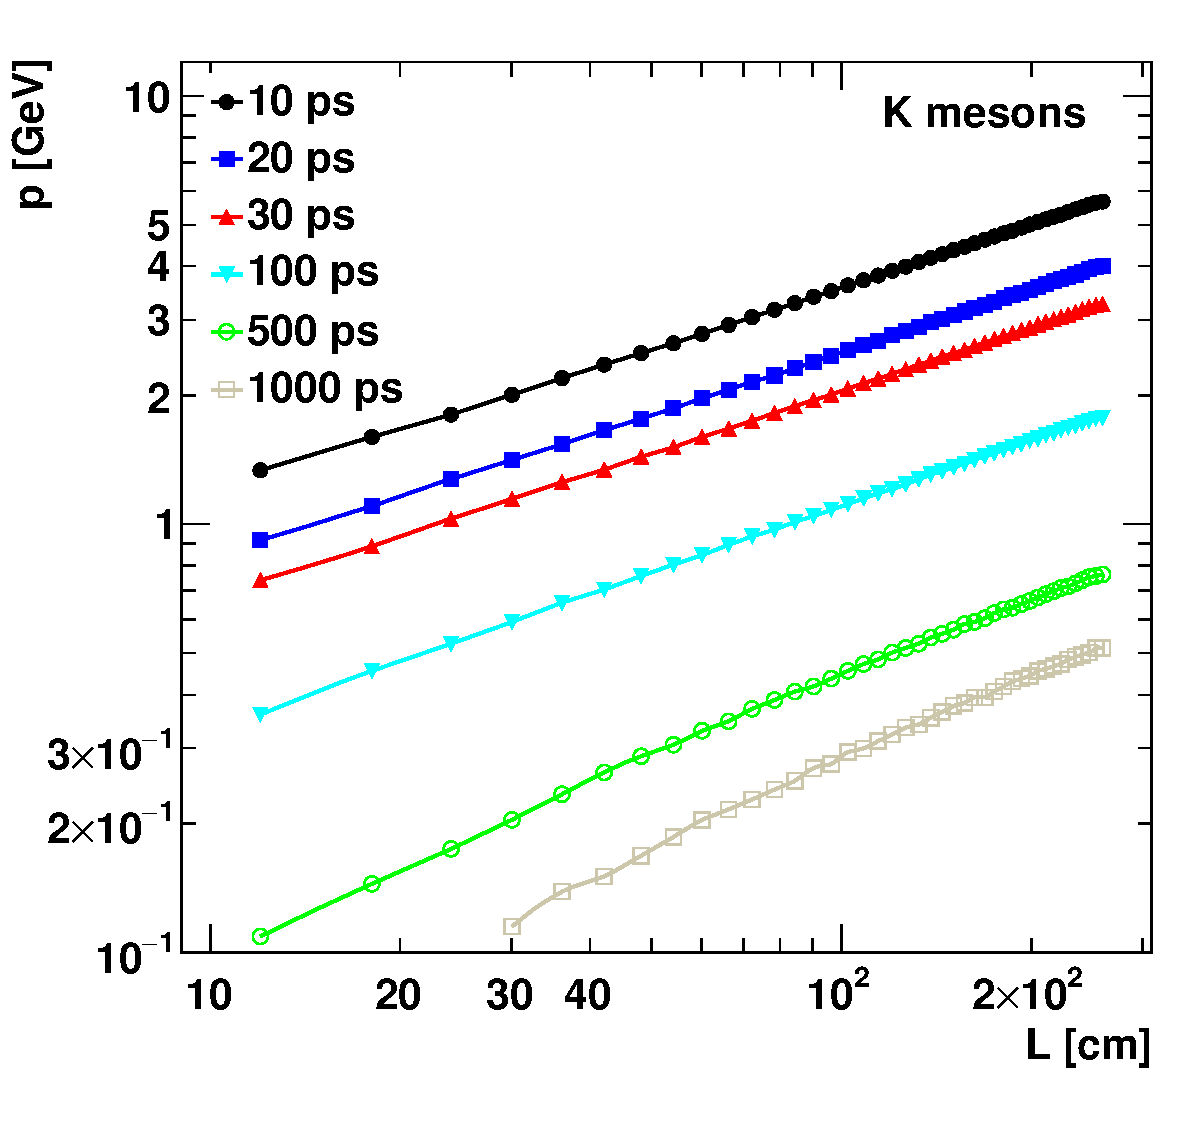
\includegraphics[width=0.45\textwidth]{time_flight_length_kion.pdf}\hfill
   }
\end{center}
\caption{
The $3\sigma$ separation from the pion-mass hypothesis for (a) neutrons and (b) kaons as a function of the length of the particle's trajectory $L$ 
and the momentum $p$. The lines show extrapolated results between the calculations indicated by the symbols.  
}
\label{fig:singleparticles}
\end{figure}


\begin{figure}
\begin{center}
   \subfigure[for $L=2$~m] {
   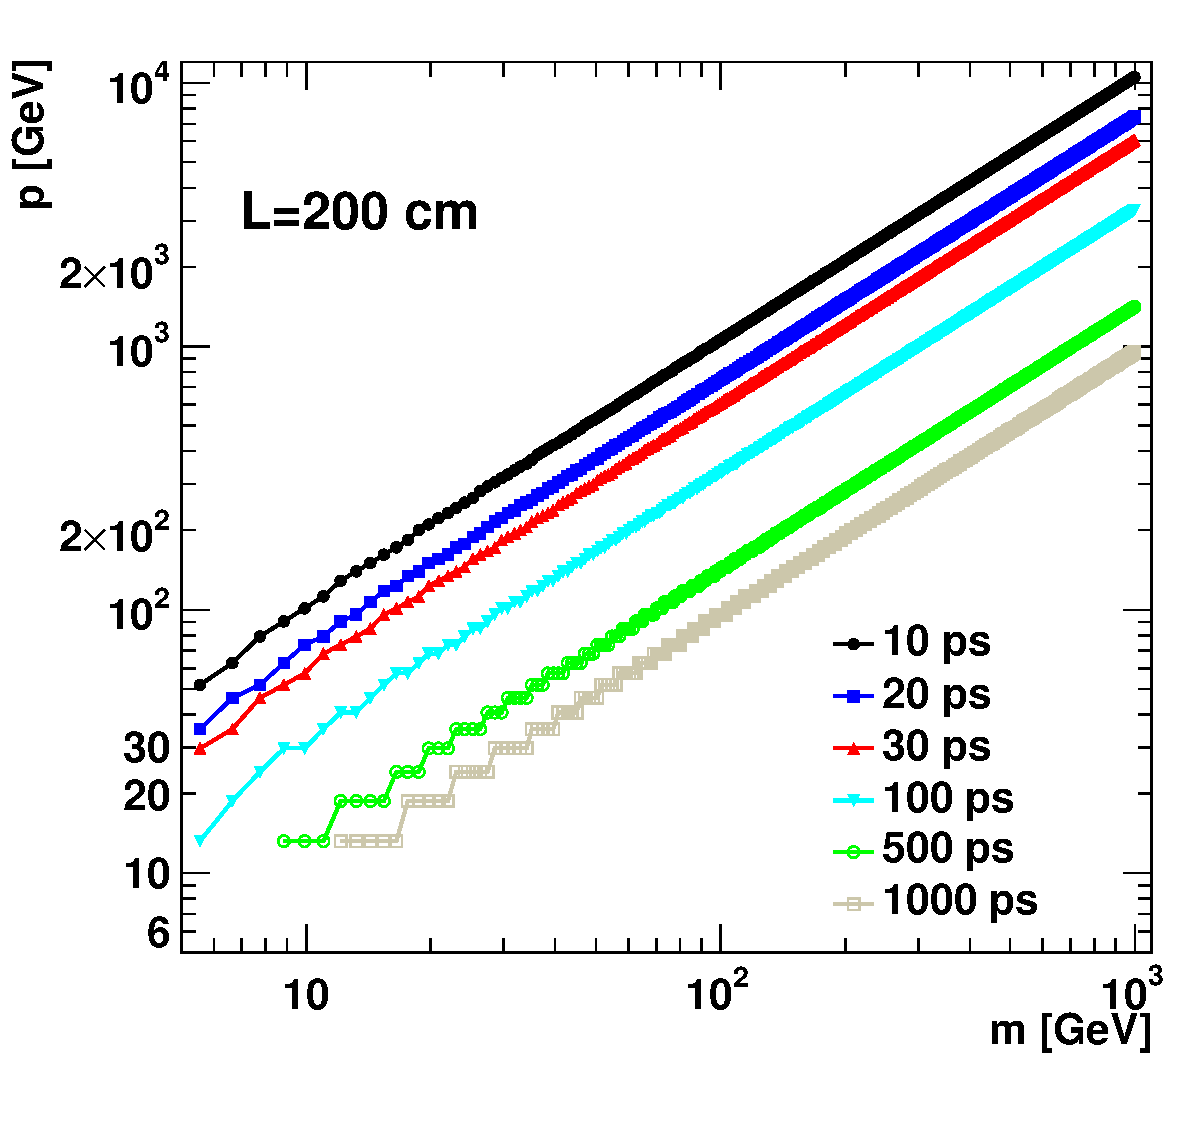
\includegraphics[width=0.45\textwidth]{time_flight_200.pdf}
   }
   \subfigure[for $L=0.2$~m] {
   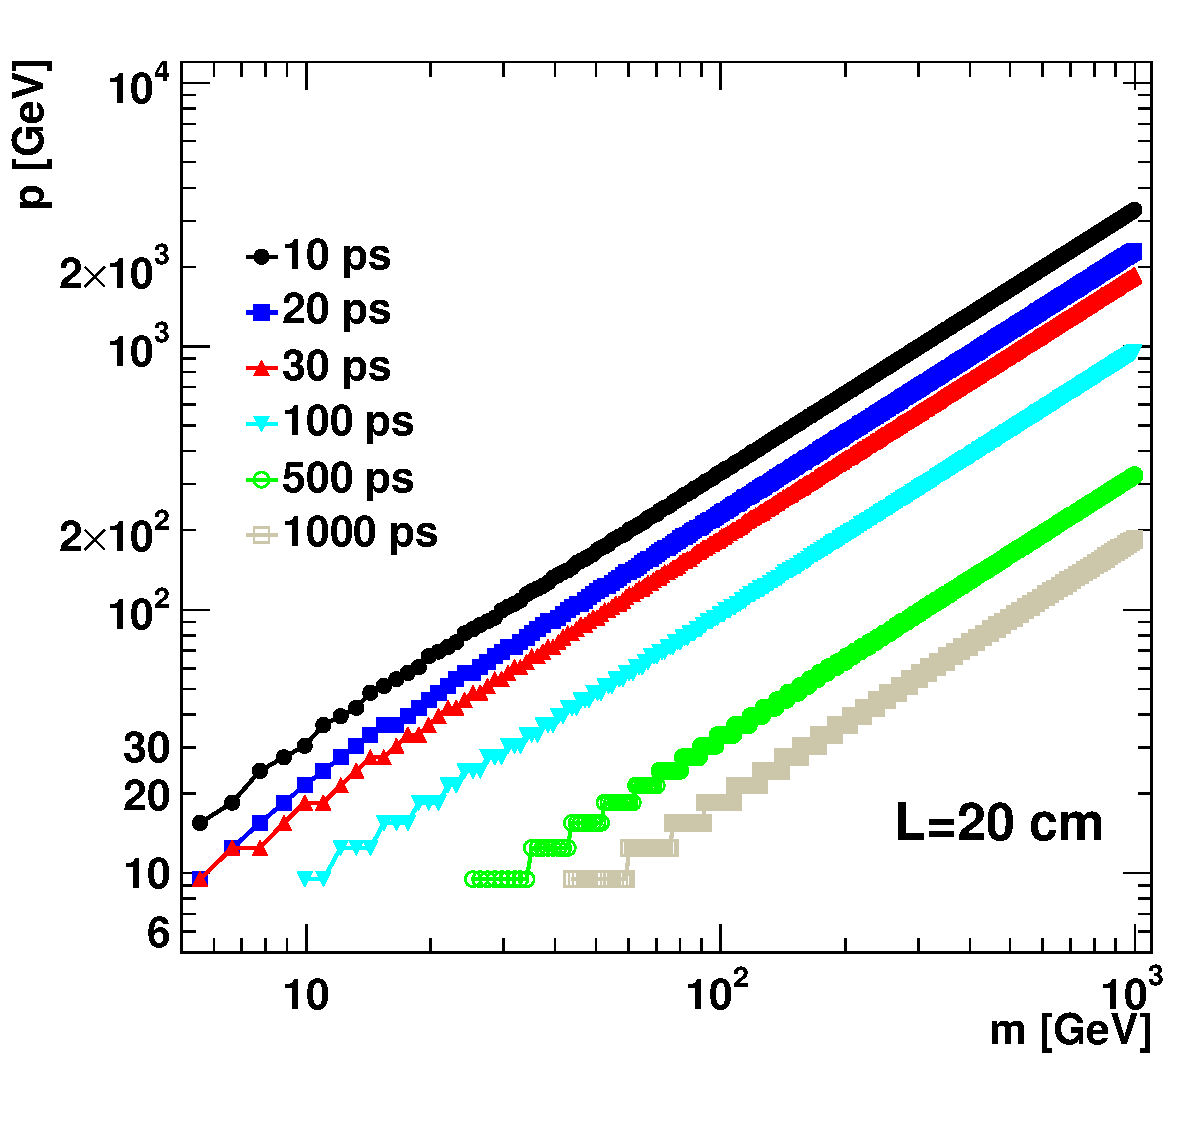
\includegraphics[width=0.45\textwidth]{time_flight_20.pdf}\hfill
   }
\end{center}
\caption{
The $3\sigma$ separation between heavy particles and $\alpha$ particles assuming timing layers with different resolutions for TOF, and using (a) $L=2$~m and (b) $L=0.2$~m.
The first value of $L$ is the typical distance
from the interaction vertex to the first layer TL1, while the second value is the typical  distance
between the two timing layers enclosing an ECAL based on the silicon technology.
}
\label{fig:signgleBSM}
\end{figure}

Having discussed the rather classical cases of discriminating  neutrons, protons and kaons from the pion hypothesis,
let us turn to the BSM searches for heavy particles.
The largest SM  backgrounds for light BSM  particles are primary protons and neutrons.
Other stable particles that can be produced by secondary interactions in the 
detector material or the beam pipe are deuterons and $\alpha$ particles. 
Although the $\alpha$ particle rate is  low since they stop easily in detector material,
it may still represent background for rare BSM particle searches.  
Therefore, we choose  $m_F=m_{\alpha}\simeq 3.73$~GeV  as reference\footnote{We clarify that the choice of $\alpha$ particles as the reference mass is
arbitrary and is only motivated by our attempt to check the $3\sigma$ separation in the momentum range $p<10$~GeV.} in  Eq.~\ref{eqTOF}, and evaluate the
$3\sigma$ separation for a wide range of masses and momenta above 4~GeV.
For many planned experiments the distance between the $pp$ collision point and the first layer of the ECAL is 
$1.5-2.5$~m. Therefore we use $L=2$~m and consider 0.2~m as the separation between the TL2 and TL1 timing layers.

Figure~\ref{fig:signgleBSM} shows the discrimination power for different choices of the timing layer resolution
and the distance $L$ (see Fig.~\ref{fig:eff_rad}).
For $L=2$~m, a stable heavy particle of mass 100~GeV can be discriminated for momentum up to 
700~GeV assuming a 20-ps timing layer,
but only up to 50~GeV using the standard 1~ns resolution.

When  TOF is measured between the layers TL1 and TL2, and assuming a spatial match of the hits, the knowledge of the interaction vertex is not required.
This type of measurement can be beneficial for neutral particles in events with large pile-up (multiple $pp$ collisions).
The identification power when $L=0.2$~m, i.e. the distance between TL2 and TL1, is shown in Fig.~\ref{fig:signgleBSM}(b).
For a stable particle with mass 100~GeV, the identification is possible up to about 200~GeV in momentum. The standard calorimeter with
1~ns resolution can only perform the identification up to $20$~GeV. 


%\section{Timing layers for ee experiments}

%%%%%%%%%%%%%%% commented out 
%\end{comment}


\section{Timing layers for FCC and jets}

%%%%%%%%%%%%%%% commented out 
%\end{comment}



\newpage
%%%%%%%%%%%%%%%%%%%%%% references %%%%%%%%%%%%%%%%%%%%%%%%%%%%%%
%\section*{References}

\bibliographystyle{elsarticle-num}
\def\bibname{\Large\bf References}
%\def\refname{\Large\bf References}
%\pagestyle{plain}
\bibliography{biblio}


\end{document}
